\documentclass[bigger]{beamer}

\usepackage{booktabs}

\usetheme{metropolis}
\metroset{block=fill}

\title{Towards Adaptive Hour of Code}

\author{Tom\'a\v{s} Effenberger\\[4mm]
%Masaryk University Brno\\
%Czech Republic

\includegraphics[width=.3\linewidth]{figures/al-logo}\\[6mm]
}

\newcommand{\img}[2]{
  \begin{center}
    \includegraphics[width=#1\linewidth]{figures/#2}
  \end{center}
}

\newcommand{\mute}[1]{
  {\color{gray}{#1}}
}


\date{AIED 2019\\Doctoral Consortium}

\begin{document}

\frame{\titlepage}
% Move to the next slide right away.

\begin{frame}
  % High-level motivation + context:
  \frametitle{Introductory Programming}

% - HoC = popular way to introduce children into programming,
%   used by millions of students every year.
% - There are many online learning systems for teaching introducotry programming;
% - and typically, they are not personalized - they offer the same sequence
%   of tasks to everybody (which necessarily leads to suboptimal learning experience).
% - Aim of the proposed research project: IP activities like HoC adaptive.

    \begin{columns}
      \column{.6\textwidth}
      \begin{center}
        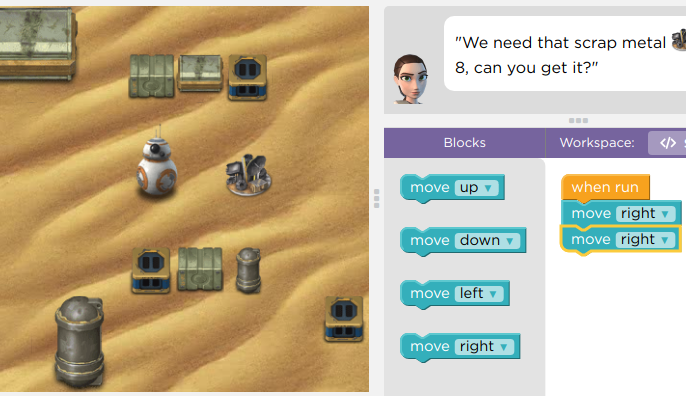
\includegraphics[width=\linewidth]{figures/hour-of-code-sw}
        \mute{https://hourofcode.com}
      \end{center}

      \column{.4\textwidth}
      \begin{center}
        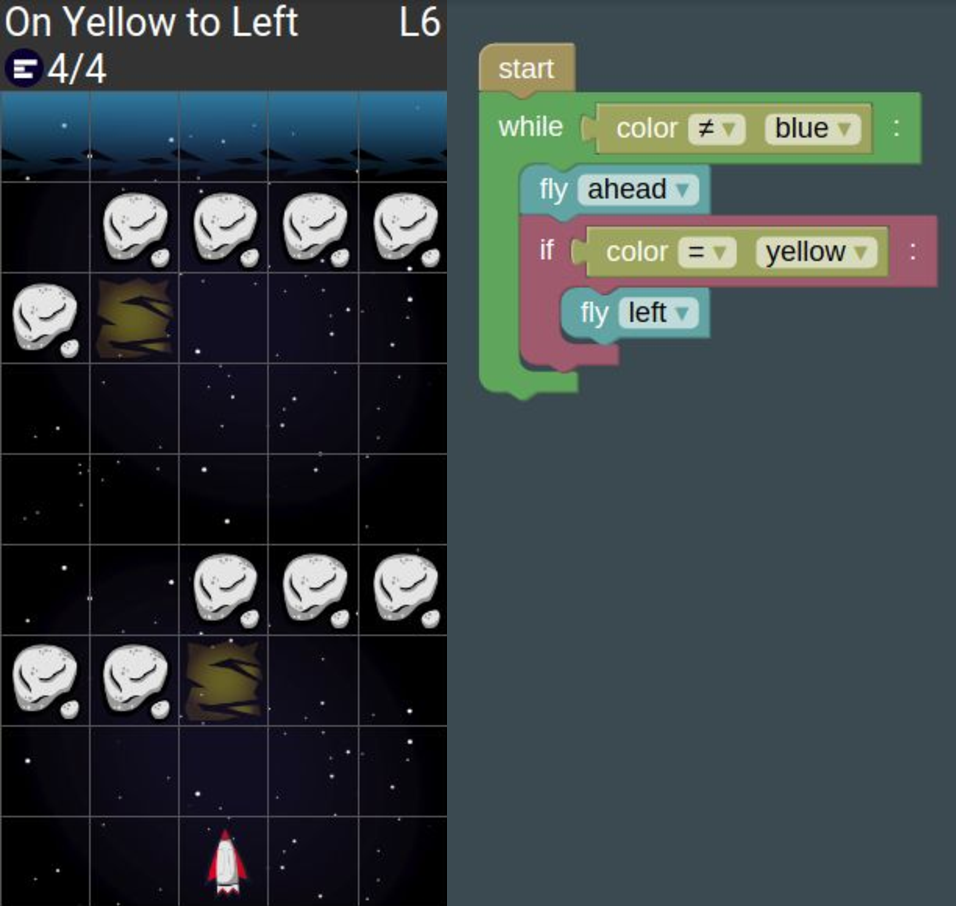
\includegraphics[width=\linewidth]{figures/robomission-on-yellow-to-left}
        \mute{https://en.robomise.cz}
      \end{center}
    \end{columns}

\end{frame}


\begin{frame}
  \frametitle{Research Questions}
  % "expected contribution to AIED" = answering these RQs

  \emph{(in the context of introductory programming)}
  % I would like to address four high-level RQs:
  % // 4 high-level RQs, one concerning DM, PM, SM, and TM.
  \begin{enumerate}
  % [domain] How to organize tasks for a personalized Hour of Code activity?
  \item How to organize tasks for a personalized Hour of Code?
        % ~ what is a suitable domain model that would facilitate a personalized behavior?
        % e.g., how to order the tasks?
        % (by HoC I don't mean only the original HoC project, but all introducotry programming
        % activities)
        % // e.g., hierarchical linearly ordered PS (our hypothesis)

  % [performance] How to measure students' performance on programming tasks?
  \item How to measure performance on programming tasks?
    % Binary success not enough.
    % Other performance aspects: time, #edits, #executions, quality of program,
    % or even the full time series of created/executed programs.

  % [student] How to predict a future performance of a student on introductory programming tasks?
  \item How to predict future performance?
  % - ... leveraging programming concepts and considering integration skills
  % - Hypothesis: For use in outer loop (online), simple model enough (if good DM and PM).
  % - // more complex model such as LogisticHMM useful for offline analysis (setting parameters).

  % Answering RQ1-3, although important on their own, are mainly steps towards RQ4.
  % [tutor] How to recommend the next task to practice in Hour of Code activities?
  \item How to recommend the next task to practice?
  % - e.g., is mastery learning appropriate and how to adapt it to non-binary
  %   performance and specific domain model?
  % - OMIT: How to introduce some safe randomization to collect diverse data useful for research
  %   while not harming the students?
  % - EXTENSION: examples illustrating concrete problems we are trying to solve (e.g.,
  % we have these three problems (and 80 more) how to order them?
  \end{enumerate}

  % - These are sort of "conventional questions" ("boring"?) but I argue, that
  %   they have not been answered sufficiently well for the context of intro
  %   programming, e.g., most research: binary performance; (only 2 problems, etc.)
  % - my goal: answer them such that the results can be applied, e.g., in Hour of Code, KA.
\end{frame}


\begin{frame}
  \frametitle{Theoretical Framework}

  % As suggested by theories of flow and ZPD, to achieve efficient learning
  % and engagement, we need to provide student with an optimal challenge.
  %state of flow,
  \begin{itemize}
  \item zone of proximal development
  % // + cognitive load theory, scaffolding

  % (NOTE: This is rather a "technical framework".)
  % But that is a difficult problem, so it is useful to decompose it into
  % several parts, e.g:
  \item models:
  \begin{itemize}
  \item domain
  \item performance
  \item student
  \item tutor
  \end{itemize}

  % These models can then be adapted to the students.
  % Adaptivity at different time scales:
  % - outer loop -- adapt to a particular student by an action (rcm) after each task
  % - design loop -- improve the whole system (adapting to a population)
  \item adaptivity:
  \begin{itemize}
  \item outer loop (mastery learning)
  \item design loop (human-in-the-loop)
  \end{itemize}
  \end{itemize}

  % Just an illustration of an example of the models currently used in RoboMission.
  % OMIT:
  % \img{0.9}{robomission-tutor-model}

\end{frame}


\begin{frame}
  \frametitle{Methods}

  \begin{itemize}
    % - In our lab, we develop two systems for teaching introductory programming,
    % - several programming exercises with tens of problems, which provides
    % me with a plenty of diverse data for exploratory analysis.
    % Multiple exercises: important for generalizability of results.
  \item exploratory analysis, multiple exercises
    \begin{itemize}
    \item robot on grid, turtle graphics, numbers/text processing
    \item interface: Blockly x Python
    \end{itemize}
    % (analysis ex: how to measure difficulty of programming tasks,
    %  how to measure similarity between tasks, how to measure performance, ...)
    % The exploratory analysis is not purely observational, because
    % we can also change the system (e.g. domain model) and evaluate
    % the intervention (design loop).

  \item online experiments to compare tutor models
    % OR: "to evaluate whether the recommendation work, whether are students learning sth"
    % "quasi-experiment?
    \begin{itemize}
    \item proxy for learning: performance on \emph{control tasks}
    \item chosen randomly after each problem set
      % Point for discussion: from which subset?
      % all tasks -> frustration; subset -> biases [transition]
    \end{itemize}

  \item simulated experiments to explore methodological issues
    % - biases: (mastery) attrition, self-selection, learning, adaptive rcm, ...
    % - to understand how can the biases influence the observed data and results
  \end{itemize}

\end{frame}


%\begin{frame}
%  \frametitle{Summary}
%  \begin{itemize}
%  % Context, Motivation: efficient & engaging HoC
%  \item adaptive learning of introductory programming
%
%  % Framework
%  \item flow, mastery learning, design loop
%
%  % Contribution to AIED: answering the research questions concerning:
%  \item domain, performance, student, and tutor modeling
%  % - in the context of introductory programming
%  % - focus on evaluation and methodological issues
%  % - mention validation of replicability ("Expected contributions" box below)
%
%  % Methods:
%  \item exploratory analysis, online and simulated experiments
%  \end{itemize}
%
%  \begin{block}{Expected contributions}
%  \begin{itemize}
%  \item recommendations on modeling approaches and evaluation methods in the
%  context of introductory programming
%  \item replicability of previous results on a broader set of exercises and problems
%  \end{itemize}
%  \end{block}
%  % Stress the number of exercises and range of problem difficulties.
%  % Request: rcmd on previous studies (both their own and from others)
%  % that they maybe don't believe and would like to know if the results
%  % generalize.
%\end{frame}


\begin{frame}
  \frametitle{Expected contributions to AIED}
  % (also serves as a summary)
  \begin{itemize}
  % Context, Motivation: efficient & engaging HoC

  \item recommendations on modeling approaches\\
        in the context of introductory programming
    % domain, performance, student, and tutor modeling
    % = ~ answering the research questions concerning
  \item focus on evaluation and methodological issues
  \item replicability of previous results on a broader set of exercises and tasks
    % Stress the number of exercises and range of problem difficulties.
    % Request: rcmd on previous studies (both their own and from others)
    % that they maybe don't believe and would like to know if the results
    % generalize.
  \end{itemize}
\end{frame}

\end{document}
